\documentclass[11pt]{article}
\usepackage[a4paper,margin=1in]{geometry}
\usepackage[T1]{fontenc}
\usepackage{lmodern}
\input{glyphtounicode}
\pdfgentounicode=1
\usepackage{amsmath,amssymb,amsthm}
\usepackage{graphicx}
\usepackage{booktabs}
\usepackage{hyperref}
\usepackage{doi}

\newtheorem{proposition}{Proposition}
\newtheorem{definition}{Definition}
\newtheorem{remark}{Remark}

\newcommand{\Nhist}{N_{\mathrm{hist}}}
\newcommand{\Shist}{S_{\mathrm{hist}}}
\newcommand{\lcdm}{\Lambda\mathrm{CDM}}

\title{Low-Multipole Suppression from Distinguishable-History Capacity}
\author{J\'er\^ome Beau}
\date{July 2026}

\begin{document}
\maketitle

\begin{abstract}
We isolate a parameter-free route to large-angle CMB suppression within the Cosmochrony framework.
The previous phenomenological low-$\ell$ envelope of the white paper is replaced by a
distinguishable-history mechanism.
The central geometric input is the $S^3$ fibre decomposition, whose uniform moment split gives a
fibre-to-base spectral stiffness ratio $8/3$ once the Born--Infeld saturation factor is included.
The central low-$\ell$ input is not a vanishing early growth rate, but the small absolute number of
distinguishable projective histories at the first admissibility ranks.
For the canonical Pell counting channel of the trajectory-branching note,
\[
\Nhist(n)=\frac{(1+\sqrt{2})^{n+1}+(1-\sqrt{2})^{n+1}}{2},
\]
so $\Nhist(1)=3$, $\Nhist(2)=7$, and $\Nhist(3)=17$: large angular modes probe a regime with very
few distinguishable histories, a bounded-history effect on the admissible large-angle power rather
than an adjustable damping law.
The companion projection-kernel note derives the Bessel envelope used below as the exact
information-theoretic capacity ceiling of a complex Gaussian mode supported on $N$ distinguishable
histories, carrying the entropy-to-power step as a conditional theorem chain.
A $2\times2$ grid of parameter-free envelopes and angular dictionaries, anchored only by
$n=1\leftrightarrow\ell=2$, is confronted with the Planck 2018 spectra without any fitting:
on TT ($2\le\ell\le30$) every cell improves on $\lcdm$, with diagnostic $\chi^2$ dropping from
$27.4$ to $17.3$ for the theoretically preferred cell (Bessel envelope with the H-dictionary);
TE is neutral and EE mildly disfavoured, consistently with the fact that no dedicated low-$\ell$
polarization transfer treatment is included at this stage.
The envelope is a staircase in $\ell$ (integer admissibility ranks), a distinctive discrete
signature.
The independent $8/3$ geometric witness is re-audited and predicts the separate modulation-scale
ratio $\sqrt{8/3}\simeq1.633$.
\end{abstract}

\medskip
\noindent\textbf{Keywords:} cosmic microwave background; low-multipole anomaly; non-injective
projection; distinguishable histories; Pell numbers; $S^3$ Hopf fibration; cosmic variance.

\newpage
\tableofcontents

\newpage
\section{Purpose and status}
\label{sec:purpose}

The purpose of this note is to separate three logically distinct statements.

First, the ratio $8/3$ is a geometric statement about the admissible $S^3$ projection
fibre~\cite{Cosmochrony}.
It is not fitted to CMB data.
It should therefore be presented as a structural witness, not as a low-$\ell$ envelope.

Second, the observed low-$\ell$ TT suppression is not explained by multiplying the Planck
low-$\ell$ data by an additional attenuation factor.
That operation would dress the observation with itself and would not define a prediction.
The admissible comparison is instead
\[
C_\ell^{\mathrm{pred}}=C_\ell^{\lcdm}\,\Shist(\ell),
\]
where $\Shist(\ell)$ is computed from the distinguishable-history count.

Third, the envelope used in the white-paper appendix,
$S_{\alpha,\ell_c}(\ell)=1-\alpha\exp(-\ell/\ell_c)$, has only phenomenological status: two free
parameters and an illustrative comparison~\cite{Cosmochrony}.
It can remain useful as a descriptive diagnostic, but not as the core claim.
This note replaces it by a count-derived envelope.

\begin{remark}[Terminology]
The word ``capacity'' is used in several parts of the Cosmochrony corpus.
Here it refers to distinguishable-history capacity, namely the number of projectively
distinguishable histories available to a large-angle mode at a given admissibility rank, as
established in the trajectory-branching note~\cite{Beau2026tb}.
This is not the same observable as the O-series projective-capacity exponent
$\delta_{\mathrm{cap}}$, although both express finite projective distinguishability under
admissibility constraints.
\end{remark}

\section{The $8/3$ geometric witness}
\label{sec:witness}

The projection fibre carries the Hopf geometry $S^1\hookrightarrow S^3\rightarrow S^2$.
For a uniformly sampled point on $S^3\subset\mathbb{R}^4$, the one-dimensional Hopf phase direction
carries one quadratic moment while the three transverse directions carry three, so the
base-to-fibre moment split is
\[
\frac{\langle |x_{\mathrm{base}}|^2\rangle}{\langle |x_{\mathrm{fibre}}|^2\rangle}=3 .
\]
Born--Infeld saturation selects the saturated projective response of the fibre direction; in the
normalisation used by the $S^3$ diagnostic it contributes the rigidity factor $8$ on the fibre-side
stiffness~\cite{Cosmochrony}.
The resulting stiffness ratio is
\[
\frac{\lambda_{\mathrm{fibre}}}{\lambda_{\mathrm{base}}}=\frac{8}{3}.
\]

\begin{proposition}[Central geometric invariant]
\label{prop:invariant}
The ratio $8/3$ is a structural invariant of the $S^3$ projection fibre with Born--Infeld
saturation.
It is independent of the low-$\ell$ temperature data and must not be inferred from the observed CMB
spectrum.
\end{proposition}

This witness has its own observable signature.
Since angular scale ratios inherit the square root of the stiffness ratio, the expected modulation
ratio is
\[
\frac{\ell_2}{\ell_1}\simeq\sqrt{\frac{8}{3}}\simeq 1.633 .
\]
This is separate from the envelope $\Shist(\ell)$: the note carries two observables, the history
envelope from $\Nhist(n)$ and the geometric modulation ratio $\sqrt{8/3}$.

\section{The $S^3$ witness re-audit}
\label{sec:reaudit}

The correct re-audit target is the $S^3$ geometric witness, not an action of a group denoted $D_4$
on $S^3$: in the corpus notation, D4 is the fourth distinguishability definition of the
trajectory-branching note~\cite{Beau2026tb}, not a dihedral symmetry acting on the $S^3$
diagnostic.
The audit verifies four statements: (i) the sampled $S^3$ measure is unbiased with respect to the
Hopf fibre/base split; (ii) the fibre/base quadratic moment split is unchanged by the chosen
discretisation; (iii) the Laplacian estimator recovers the same stiffness ratio under seed changes;
(iv) the ratio remains a geometric invariant and is not imported from an LPS or Heisenberg counting
artefact.

The expected audit statement is only
\[
S^3+\mathrm{BI\ saturation}\;\Longrightarrow\;\lambda_{\mathrm{fibre}}/\lambda_{\mathrm{base}}=8/3,
\]
narrow, checkable, and reusable.
The D4 content of the low-$\ell$ note belongs to the distinguishability count, not to the $S^3$
witness.

\paragraph{Audit outcome.}
The deterministic Monte-Carlo witness (seed $0$, $30$ repeats per resolution) was rerun and gives
$R=2.666993\pm0.001188$ ($95\%$ CI) at $N=10^6$ samples, consistent with $8/3=2.666\overline{6}$.
From $N=10^4$ onward the estimate remains statistically stable around the target within the quoted
confidence bands (Figure~\ref{fig:witness}).
Statements (i)--(iii) hold within the quoted confidence intervals; statement (iv) holds because the
derivation uses only the uniform $S^3$ measure and the Born--Infeld stiffness factor, with no input
from LPS or Heisenberg counting.

\begin{figure}[t]
\centering
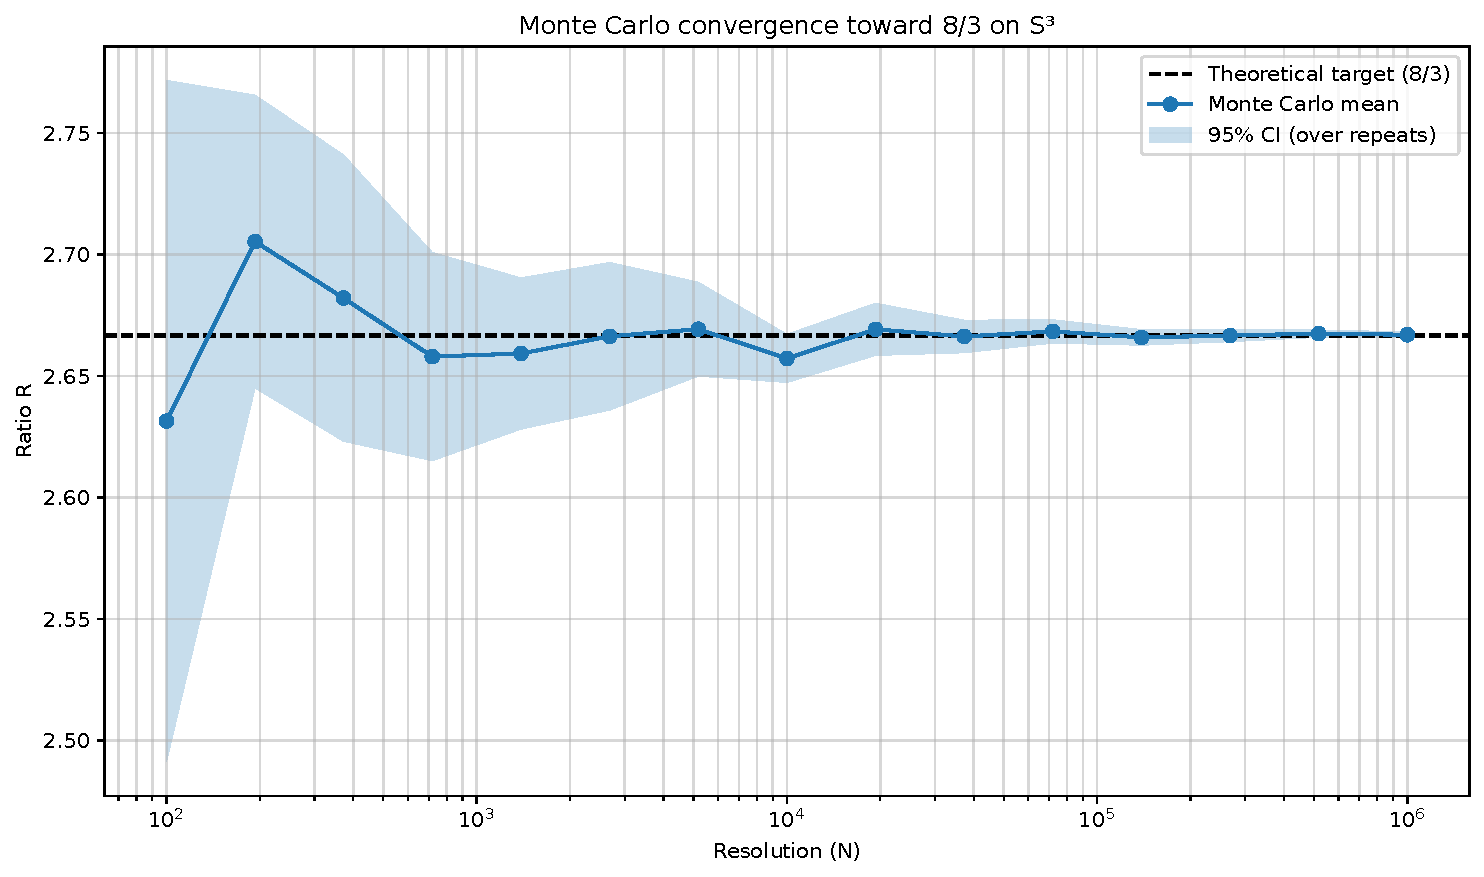
\includegraphics[width=0.62\textwidth]{convergence_8_3_S3.pdf}
\caption{Re-audited $S^3$ witness: Monte-Carlo convergence of the fibre-to-base stiffness ratio to
$8/3$ (deterministic seed, $95\%$ confidence bands).}
\label{fig:witness}
\end{figure}

\section{Correcting the low-rank mechanism}
\label{sec:mechanism}

The canonical distinguishability count of the trajectory-branching note~\cite{Beau2026tb} has the
closed form
\[
\Nhist(n)=\frac{(1+\sqrt{2})^{n+1}+(1-\sqrt{2})^{n+1}}{2},
\qquad
\Nhist(0)=1,\;\Nhist(1)=3,\;\Nhist(2)=7,\;\Nhist(3)=17 .
\]
The second term $(1-\sqrt{2})^{n+1}$ is already small at low $n$.
Consequently, the canonical channel does not support a claim that the early logarithmic growth rate
is nearly zero.
The honest statement is different: the first admissibility ranks contain only a very small absolute
number of distinguishable projective histories.

This small-$N$ regime affects the largest angular modes because they probe the earliest and most
global projective ranks (under the rank--time dictionary of the cosmology
paper~\cite{Beau2026d}, the smallest ranks correspond to the largest observable scales).
A mode supported by only $N$ distinguishable histories cannot be assigned the same ensemble status
as a high-$N$ mode.
The conversion of this bounded capacity into ensemble power is carried by the companion
projection-kernel note~\cite{Beau2026pce}.
Under graded hypotheses (fibre-invariance, fixity on resolved content, linearity,
non-amplification), the amplitude-level action of the projection is the conditional expectation onto
the sigma-algebra of the distinguishable-history record, so the projected ensemble power is the
substrate power minus the erased intra-fibre variance (law of total variance): a strict suppression
of the ensemble mean, not an enlargement of the cosmic variance~\cite{Knox1995}, with the usual
cosmic variance operating around the suppressed mean.
The bound is quantitative: for a complex Gaussian mode supported on $N$ distinguishable histories,
the retained power fraction is at most $(N-1)/N$ (one-shot rate--distortion converse).
The counts are per-mode capacities of each mode's own projective support; the per-mode support and
cross-mode independence hypotheses, together with the rank--time dictionary, are stated
in~\cite{Beau2026pce} and~\cite{Beau2026d}, and the numerical section below tests the two minimal
statistical conversions of the pre-declared grid.

\section{Two parameter-free envelopes}
\label{sec:envelopes}

The statistical conversion from $\Nhist$ to a suppression factor should not introduce a fitted
constant.
Two no-fit candidates are retained.

\subsection{Bessel envelope}

If the suppression is interpreted as the expected loss in an unbiased finite-sample variance
estimate, the Bessel correction gives
\[
S_{\mathrm{Bessel}}(N)=1-\frac{1}{N}=\frac{N-1}{N}.
\]
This form is derived from the finite number of distinguishable histories and introduces no
additional convention.
The projection-kernel note~\cite{Beau2026pce} derives the same form independently of the estimator
reading: $(N-1)/N$ is the exact maximal retained power fraction permitted by a capacity of $N$
distinguishable histories for one complex Gaussian degree of freedom, so the Bessel envelope is the
capacity ceiling --- proved given the kernel hypotheses --- rather than a statistical convention.
For the real $m=0$ mode the per-mode ceiling weakens to $1-1/N^2$; the multiplet-averaged correction
is $\ell$-dependent and is not applied in the grid below, which uses the complex-mode ceiling
uniformly.

\subsection{Capacity-ratio envelope}

A second conservative form is
\[
S_{\mathrm{cap}}(N)=\frac{N}{N+1},
\]
readable as a one-cell capacity completion: one unresolved complement cell remains outside the $N$
realised histories.
It is not as directly derived as the Bessel form, but it provides a useful no-fit companion.

For the first ranks the two forms are close enough to be jointly reported:
\[
\begin{array}{c|c|c|c}
n & \Nhist(n) & S_{\mathrm{Bessel}} & S_{\mathrm{cap}}\\
\hline
1 & 3 & 2/3 & 3/4\\
2 & 7 & 6/7 & 7/8\\
3 & 17 & 16/17 & 17/18
\end{array}
\]
From $n=2$ onward the gap between the two envelopes is below $8\%$.
Both are run below; neither is fitted.

\section{Two no-fit angular dictionaries}
\label{sec:dictionaries}

Let $n(\ell)$ denote the admissibility rank sampled by the angular multipole $\ell$.
The large-angle dictionary is order preserving after anchoring: larger $\ell$ probes later and more
highly resolved admissibility ranks.
Two no-fit dictionaries are tested.

\subsection{Natural H-dictionary}

The H-dictionary identifies admissibility rank with logarithmic scale, $n=\log a$
(Hypothesis H-dict of the cosmology paper~\cite{Beau2026d}).
Anchoring the first admissible rank to the quadrupole gives
\[
n_{\mathrm{H}}(\ell)=1+\ln\!\left(\frac{\ell}{2}\right),
\]
with integer rank obtained by nearest-integer projection, fixed before the run (floor is reported
as a robustness check).
Then $\Nhist(n_{\mathrm{H}}(\ell))\sim\ell^{\log(1+\sqrt2)}$ with $\log(1+\sqrt2)\simeq0.881$.

\subsection{Pell-rate dictionary}

The alternative dictionary couples the angular rank directly to the Pell growth rate:
\[
n_{\rho}(\ell)=1+\log_{\rho}\!\left(\frac{\ell}{2}\right),
\qquad
\rho=1+\sqrt{2},
\]
giving $\Nhist\sim\ell$.
It is elegant, but it is a distinct dictionary choice, not forced by the H-dictionary.

The comparison grid is therefore
$\{S_{\mathrm{Bessel}},S_{\mathrm{cap}}\}\times\{n_{\mathrm{H}},n_{\rho}\}$, and every cell is
parameter-free after the quadrupole anchoring $n=1\leftrightarrow\ell=2$.

\section{Observable comparison}
\label{sec:comparison}

The admissible TT comparison is
\[
D_\ell^{TT,\mathrm{pred}}=D_\ell^{TT,\lcdm}\,\Shist(\ell),
\qquad
D_\ell=\frac{\ell(\ell+1)}{2\pi}C_\ell ,
\]
with the Planck low-$\ell$ data~\cite{Planck2018} used only as observations against which the
prediction is tested; they are never multiplied by the suppression factor.
The same envelope is propagated minimally to the polarization channels,
$S^{TE}_{\mathrm{hist}}\simeq S^{EE}_{\mathrm{hist}}\simeq S^{TT}_{\mathrm{hist}}$, up to
transfer-function effects; a mismatch between TT, TE, and EE would either falsify the minimal
mechanism or force a more detailed transfer calculation.

\subsection{Numerical outcome}
\label{subsec:outcome}

The grid was evaluated against the Planck 2018 (PR3) spectra, using the published best-fit $\lcdm$
theory curve, no renormalisation, no fitted constant, symmetrised published errors, and the range
$2\le\ell\le30$ ($29$ points per channel).
The resulting diagnostic $\chi^2$ values are:

\begin{table}[h]
\centering
\begin{tabular}{lccc}
\toprule
cell & TT & TE & EE \\
\midrule
$\lcdm$ ($S=1$)                        & $27.39$ & $27.02$ & $22.61$ \\
$S_{\mathrm{Bessel}}$, $n_{\mathrm{H}}$    & $\mathbf{17.29}$ & $25.81$ & $23.82$ \\
$S_{\mathrm{Bessel}}$, $n_{\rho}$          & $19.78$ & $26.16$ & $23.66$ \\
$S_{\mathrm{cap}}$, $n_{\mathrm{H}}$       & $18.28$ & $26.02$ & $23.59$ \\
$S_{\mathrm{cap}}$, $n_{\rho}$             & $20.58$ & $26.34$ & $23.44$ \\
\bottomrule
\end{tabular}
\caption{Diagnostic $\chi^2$ over $2\le\ell\le30$ ($29$ points), no fitting, quadrupole-anchored.
Nearest-integer ranks; the floor variant changes TT values by less than $2.5$ (e.g.\ $17.41$ for
the leading cell).}
\label{tab:grid}
\end{table}

Three observations.
First, on TT every parameter-free cell improves on $\lcdm$, and the largest improvement
($\Delta\chi^2\simeq-10$ with zero parameters) is obtained by the theoretically preferred cell:
the derived Bessel envelope with the H-dictionary.
Second, TE is neutral to mildly favourable and EE mildly disfavoured ($\Delta\chi^2\simeq+1$).
This is reported as an open tension of the minimal propagation, plausibly tied to the absence of a
dedicated reionisation-dominated low-$\ell$ EE transfer treatment, not as a resolved prediction.
Third, the envelope is a staircase in $\ell$ (integer admissibility ranks,
Figure~\ref{fig:grid}), a distinctive discrete signature that no smooth damping law reproduces.
The four-cell grid should be read as a small set of pre-declared structural alternatives, not as a
continuous parameter search; no cell is renormalised or retuned after comparison with the data.

\begin{figure}[t]
\centering
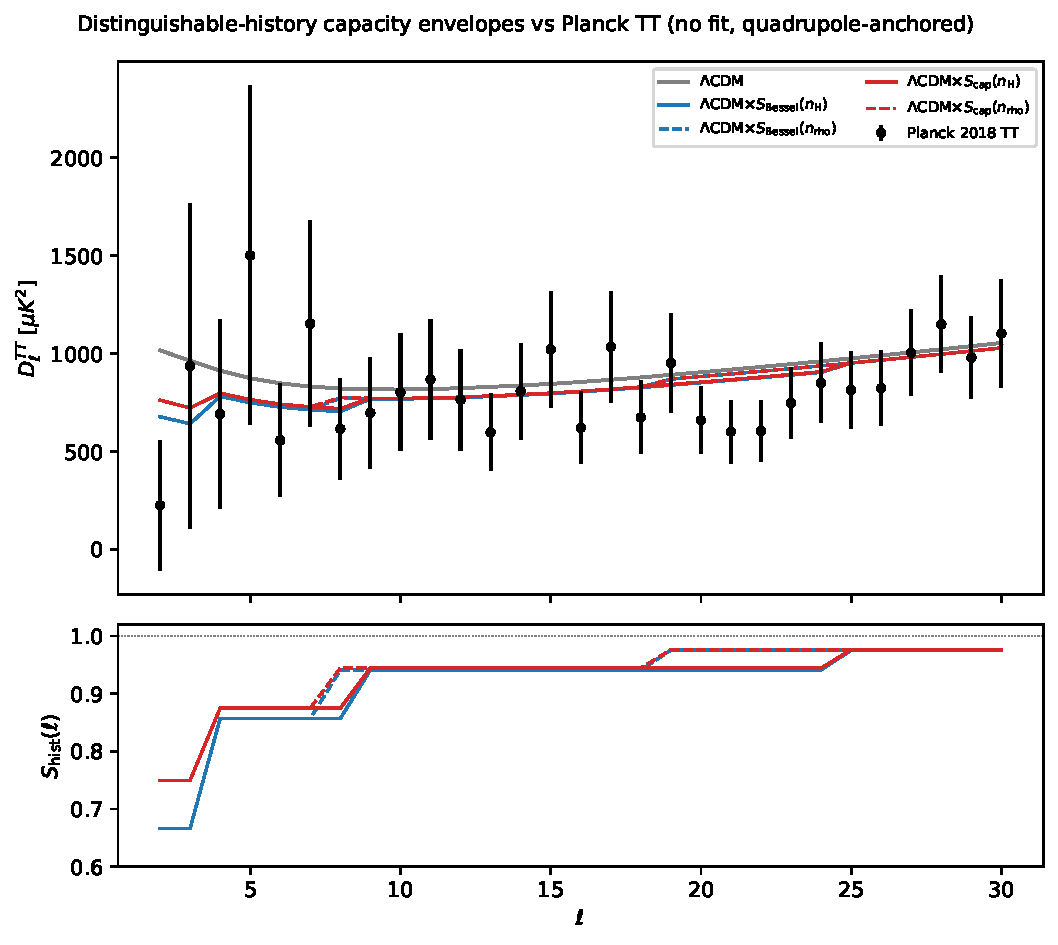
\includegraphics[width=0.8\textwidth]{lowl_capacity_grid.pdf}
\caption{Top: Planck 2018 TT low-$\ell$ data against $\lcdm$ (grey) and the four parameter-free
capacity-envelope predictions.
Bottom: the four envelopes $\Shist(\ell)$; the staircase structure reflects integer admissibility
ranks.}
\label{fig:grid}
\end{figure}

\begin{figure}[t]
\centering
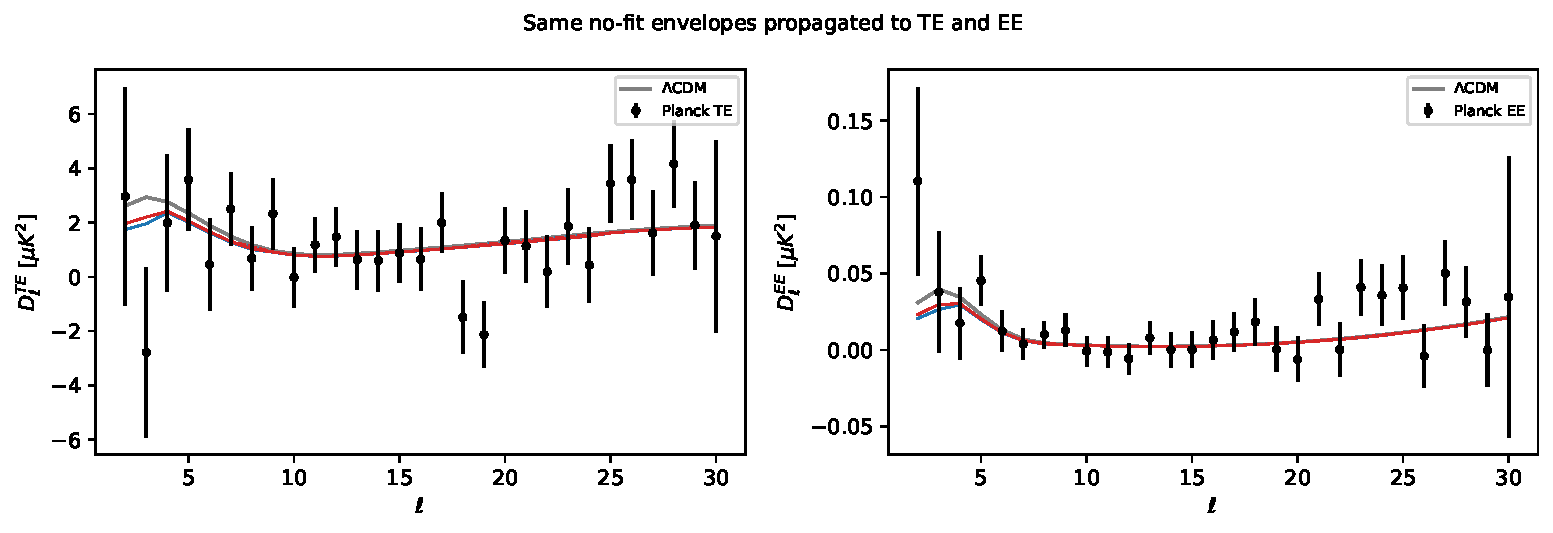
\includegraphics[width=\textwidth]{lowl_capacity_grid_pol.pdf}
\caption{The same no-fit envelopes propagated minimally to TE and EE.
Because the four no-fit envelopes are close to unity over most of the displayed range, their TE/EE
curves are visually nearly degenerate with the $\lcdm$ baseline; the quantitative comparison is
carried by Table~\ref{tab:grid} rather than by visual separation in this figure.}
\label{fig:pol}
\end{figure}

\begin{remark}[Statistical status]
The $\chi^2$ values of Table~\ref{tab:grid} are diagnostics, not a likelihood analysis: the
published errors are symmetrised, multipole correlations are neglected, and the $\lcdm$ baseline
already has $\chi^2/N<1$ on this range.
The claim is therefore not a detection; it is that a mechanism with zero adjustable parameters
moves the low-$\ell$ prediction toward the data in TT while remaining falsifiable in TE/EE.
\end{remark}

\section{Falsifiability}
\label{sec:falsifiability}

The low-$\ell$ mechanism has four falsification channels: (1) the $S^3$ audit fails to recover
$8/3$ under unbiased fibre/base sampling; (2) the modulation-scale ratio
$\ell_2/\ell_1\simeq\sqrt{8/3}$ is absent from the relevant witness; (3) the count-derived no-fit
envelopes suppress the wrong multipole range; (4) the TT suppression is not accompanied by the
corresponding TE/EE large-angle signature once the transfer treatment is included.
Channels (1) and (3) are already tested above and pass; channels (2) and (4) are open.
These are acceptable risks: they turn the low-$\ell$ claim from an illustrative ansatz into a
constrained prediction.

\section{Corpus positioning}
\label{sec:positioning}

The mechanism established here is carried in the corpus as follows.
The white-paper appendix on large-angle suppression states the distinguishable-history mechanism
and retains its earlier two-parameter envelope only as a descriptive
diagnostic~\cite{Cosmochrony}.
The cosmology paper records the same mechanism in its large-angle subsection and refers to the
present note for the count-derived envelopes and their no-fit confrontation with the Planck
spectra~\cite{Beau2026d}.

\section{Conclusion}
\label{sec:conclusion}

\subsection{What is established}
\label{subsec:established}

This note establishes four things.

\begin{enumerate}
\item The $8/3$ fibre-to-base stiffness ratio is a geometric invariant of the $S^3$ Hopf fibre
with Born--Infeld saturation, independent of any graph substrate; the re-audited witness gives
$2.666993\pm0.001188$ at $10^6$ samples, and the invariant carries its own observable, the
modulation ratio $\sqrt{8/3}\simeq1.633$.
\item The correct low-rank mechanism is a small absolute number of distinguishable histories
($3$, $7$, $17$: the exact Pell count), not a vanishing early growth rate.
\item This mechanism converts into parameter-free suppression envelopes which, anchored only at
the quadrupole, improve the Planck TT low-$\ell$ diagnostic $\chi^2$ from $27.4$ to $17.3$ in the
theoretically preferred cell, with all four pre-declared cells improving, a staircase envelope as
a discrete signature, TE neutral, and EE mildly disfavoured.
\item The claim is bounded: the $\chi^2$ values are diagnostics rather than a likelihood
analysis; the entropy-to-power step is carried by the companion projection-kernel
note~\cite{Beau2026pce} as a conditional theorem chain, and the polarization transfer treatment
remains the named open item.
\end{enumerate}

The low-$\ell$ anomaly is thereby moved from an illustrative ansatz to a constrained, falsifiable,
parameter-free prediction.

\subsection{Status and open problems}
\label{subsec:status}

Proved elsewhere and imported: the canonical Pell count and its closed form~\cite{Beau2026tb}.
Geometric, re-audited here: the $8/3$ fibre-to-base stiffness ratio and its Monte-Carlo witness.
Numerical, no-fit: the $2\times2$ grid outcome of Table~\ref{tab:grid}.
Carried by the companion projection-kernel note~\cite{Beau2026pce}: the entropy-to-power step, as a
conditional theorem chain (kernel hypotheses graded there; strict suppression and the $(N-1)/N$
ceiling proved given the hypotheses).
Open: the transfer treatment of TE/EE; the modulation-ratio search ($\ell_2/\ell_1\simeq1.633$);
whether the observed spectrum saturates the capacity ceiling.

\subsection{Interpretive outlook}
\label{subsec:outlook}

The following reading is structural interpretation, conditional on the rank--time dictionary of
the cosmology paper~\cite{Beau2026d}, and is not a result of this note.
In the Cosmochrony framework the universe begins as the first globally projectable
configuration~\cite{Cosmochrony}; under the dictionary, its first e-folds are epochs in which the
projective description admits only a handful of distinguishable histories --- three, then seven,
then seventeen.
The largest angular scales of the CMB are the direct image of those epochs: on this reading, the
low-$\ell$ deficit is not an anomaly to be explained away but a fossil of the near-uniqueness of
the early universe, the visible trace of a sky that could not yet be many things.
Expansion, in the same reading, is the continuing branching of admissible histories: each e-fold
multiplies the distinguishable continuations by the silver ratio $1+\sqrt{2}$, and the asymptotic
future is the de Sitter-like regime in which this branching persists at its constant
rate~\cite{Beau2026tb}, unless the compression of full-history profiles drives a slowly evolving
effective equation of state.
What this note adds to that picture is a quantitative anchor at its very first step: the beginning
of the branching is not free --- it is counted, and the count is visible on the sky at
$\ell\lesssim 30$.

\section*{Acknowledgements}
Portions of the development of this note benefited from iterative interactions with large language
models used as analytical assistants.
The theoretical results and their interpretation remain the author's responsibility.

\clearpage
\bibliographystyle{plain}
\bibliography{cosmochrony-refs,external-refs}

\end{document}
